\chapter{Preparation}

This chapter introduces Prolog and WebAssembly, as well as giving an overview of garbage collection techniques to be explored in the project. It also describes the tools and development methodology used in the implementation of the Prolog interpreter. Finally, it states the starting point of the project.

\section{Prolog}

Prolog is rooted in the fundamental idea that logic can be used as a programming language \cite{kowalskiPredicateLogicProgramming1974}. This section summarises the theory behind Prolog, as well as its execution model and practical implementation details.

\subsection{First-Order Logic}

Prolog is based on \emph{first-order logic}, which is a formal system for reasoning about statements that can be true or false.

In first-order logic, terms, formulas, and clauses are built up from an alphabet of \emph{variables} $x, y, z$, \emph{function symbols} $f, g, h$, and \emph{predicate symbols} $P, Q, R$. Function and predicate symbols have an associated \emph{arity}. A $0$-ary function symbol is called a \emph{constant}.

\begin{definition}
A \emph{term} is inductively defined as follows:
\begin{itemize}
\item A variable is a term.
\item If $t_1, \ldots, t_n$ are terms and $f$ is an $n$-ary function symbol, then $f(t_1, \ldots, t_n)$ is a term.
\end{itemize}
\end{definition}

\begin{definition}
A \emph{formula} is inductively defined as follows:
\begin{itemize}
\item If $t_1, \ldots, t_n$ are terms and $P$ is an $n$-ary predicate symbol, then $P(t_1, \ldots, t_n)$ is an \emph{atomic formula}, or \emph{atom}.
\item If $A$ is a formula, then $\neg A$ is a formula.
\item If $A$ and $B$ are formulas, then $A \land B$, $A \lor B$, $A \rightarrow B$, and $A \leftrightarrow B$ are formulas.
\item If $A$ is a formula and $x$ is a variable, then $\forall x A$ and $\exists x A$ are formulas.
\end{itemize}
\end{definition}

\begin{definition}
A \emph{literal} is an atomic formula (a \emph{positive literal}) or the negation of an atomic formula (a \emph{negative literal}).
\end{definition}

\begin{definition}
A \emph{clause} is a universally quantified disjunction of literals
$$
\forall x_1, \ldots, x_s (L_1 \lor \ldots \lor L_k)
$$
where $x_1, \ldots x_s$ are variables appearing in the literals $L_1, \ldots, L_m$. The positive literals $B_i$ may also be separated from the negative literals $A_i$, the universal quantification made implicit, and the clause written as
$$
B_1 \lor \ldots \lor B_n \leftarrow A_1 \land \ldots \land A_m
$$
\end{definition}

\begin{definition}
A \emph{Horn clause} is a clause with at most one positive literal.
$$
B \leftarrow A_1 \land \cdots \land A_m
$$
A clause with exactly one positive literal is called a \emph{definite clause}, and a clause with no positive literals is called a \emph{goal clause} or \emph{goal}.
\end{definition}

\subsection{Unification}

\emph{Unification} is the process of finding a \emph{substitution} that makes two terms equal. A substitution $\theta$ is a set of variable assignments, written $[t_1/x_1, \ldots, t_n/x_n]$, where $t_i$ are terms and $x_i$ distinct variables. A substitution is a \emph{unifier} of two terms $t_1$ and $t_2$ if $t_1\theta = t_2\theta$. The \emph{most general unifier} (MGU) $\theta$ of two terms is a unifier that is more general than any other unifier, that is, all other unifiers $\phi$ can be written as the composition of $\theta$ and another substitution $\psi$.

\paragraph{Martelli-Montanari Algorithm}

The \emph{Martelli-Montanari algorithm} is an algorithm for computing the most general unifier of two terms $t_1$ and $t_2$ \cite{martelliEfficientUnificationAlgorithm1982}. It iteratively applies rules to a set of equations, starting with $\{t_1 = t_2\}$, until no more rules can be applied, at which point the set of equations is the unifier.

The rules are shown in Figure \ref{fig:martelli-montanari}. $s$ and $t$ are terms, $X$ and $Y$ are variables, $f$ and $g$ are function symbols, and $S$ is a set of equations. $\text{vars}(t)$ denotes the set of variables occurring in $t$.

\begin{figure}[H]
\begin{align*}
\{f(s_1, \ldots, s_n) = f(t_1, \ldots, t_n)\} \cup S &\rightarrow \{s_1 = t_1, \ldots, s_n = t_n\} \cup S \\
\{f(s_1, \ldots, s_n) = g(t_1, \ldots, t_m)\} \cup S &\rightarrow \text{fail} \\
\{X = X\} \cup S &\rightarrow S \\
\{X = t\} \cup S &\rightarrow \{X = t\} \cup S[t/X] \quad \text{if } X \notin \text{vars}(t) \\
\{X = t\} \cup S &\rightarrow \text{fail} \quad \text{if } X \in \text{vars}(t) \land X \neq t
\end{align*}
\caption{The Martelli-Montanari algorithm}
\label{fig:martelli-montanari}
\end{figure}

The condition $X \notin \text{vars}(t)$ is called the \emph{occurs check}, and is included to prevent the creation of infinite terms. In Prolog, the occurs check is often disabled by default for performance reasons, which enables the representation of cyclic terms.

\subsection{Resolution}

\emph{Resolution} enables the inference of new clauses from existing clauses. In particular, the more restrictive \emph{SLD resolution} (selective linear definite resolution) is the basis of Prolog's execution model.

Given a goal clause $\neg A_1 \lor \cdots \lor \neg A_n$, and a definite clause $B \lor \neg B_1 \lor \cdots \lor \neg B_m$, such that $B$ and some $A_i$ unify with MGU $\theta$, a new goal clause can be derived by applying the resolution rule:
$$
\frac{B \lor \neg B_1 \lor \cdots \lor \neg B_m \qquad \neg A_1 \lor \cdots \lor \neg A_n}{(\neg A_1 \lor \cdots \lor \neg A_{i-1} \lor \neg A_{i+1} \lor \cdots \lor \neg A_n \lor \neg B_1 \lor \cdots \lor \neg B_m)\theta}
$$

\subsection{Logic Programming}

A key insight of Kowalski's \emph{logic programming} paradigm is that all questions concerning logical implication in first-order logic can be equivalently stated as questions of satisfiability of sentences in \emph{clausal form} \cite{kowalskiPredicateLogicProgramming1974}. Furthermore, it is sufficient to limit ourselves to Horn clauses \cite{hillLUSHresolutionitscompleteness1974}, which we can interpret as procedures of a simple programming language, with procedure invocation corresponding to SLD resolution.

\paragraph{Example}

To illustrate this idea, consider the following logical implication, which asks whether there exists an $x$ such that $x$ is the factorial of 2. We assume the existence of a ternary predicate \texttt{times} that relates the pair $(x, y)$ to its product.
\begin{gather*}
\texttt{fact}(0, s(0)) \quad \land \quad \forall x (\texttt{fact}(x, v) \land \texttt{times}(s(x), v, w) \rightarrow \texttt{fact}(s(x), w)) \\
\rightarrow \exists x \ \texttt{fact}(s(s(0)), x)
\end{gather*}

It is equivalent to ask whether the following Horn clauses are satisfiable, that is, whether there exists some substitution that makes the conjunction of the clauses true in first-order logic.

\begin{align*}
\{ \qquad & \texttt{fact}(0, s(0)), \\
& \texttt{fact}(s(x), w) \leftarrow \texttt{fact}(x, v) \land \texttt{times}(s(x), v, w), \\
& \leftarrow \texttt{fact}(s(s(0)), x) & \}
\end{align*}

Written in Prolog syntax, the corresponding program is as follows.

\begin{center}
\begin{minted}{prolog}
fact(0, s(0)).
fact(s(X), W) :- fact(X, V), times(s(X), V, W).
?- fact(s(s(0)), X).
\end{minted}
\end{center}

\subsection{Execution Model}

SLD resolution implicitly constructs a \emph{search tree} of possible substitutions, and the execution model of Prolog can be understood as a depth-first search of this tree. Consider the following Prolog program.

\begin{center}
\begin{minted}{prolog}
king(united_kingdom, charles).
king(denmark, frederik).
country(united_kingdom).
country(france).
country(denmark).

?- country(C), king(C, K).
\end{minted}
\end{center}

The execution of this program explores the search tree shown in Figure \ref{fig:prolog-search-tree}.

\begin{figure}[H]
\begin{center}
  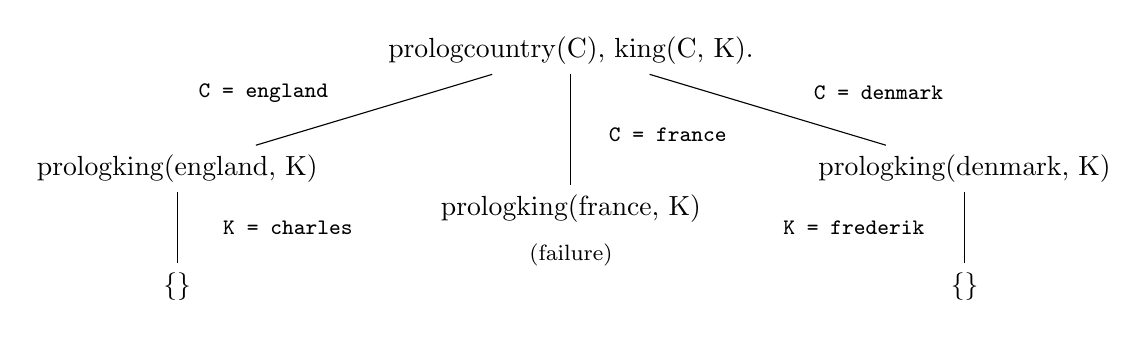
\begin{tikzpicture}
      \node (A) at (0,3) {\mintinline{prolog}{country(C), king(C, K).}};
      \node (B1) at (-5,1.5) {\mintinline{prolog}{king(england, K)}};
      \node (B2) at (0,1) {\mintinline{prolog}{king(france, K)}};
      \node (B3) at (5,1.5) {\mintinline{prolog}{king(denmark, K)}};
      \node (C1) at (-5,0) {\{\}};
      \node (C2) at (5,0) {\{\}};

      \draw (A) -- (B1) node [midway, xshift=-40, yshift=6] {\footnotesize \texttt{C = england}};
      \draw (A) -- (B2) node [midway, xshift=35, yshift=-2] {\footnotesize \texttt{C = france}};
      \draw (A) -- (B3) node [midway, xshift=40, yshift=6] {\footnotesize \texttt{C = denmark}};
      \draw (B1) -- (C1) node [midway, xshift=40] {\footnotesize \texttt{K = charles}};
      \draw (B3) -- (C2) node [midway, xshift=-40] {\footnotesize \texttt{K = frederik}};

      \node (D) at (0,0.4) {\footnotesize (failure)};
  \end{tikzpicture}
\end{center}
\caption{Search tree for the Prolog program}
\label{fig:prolog-search-tree}
\end{figure}

The tree is searched depth-first, left-to-right, with clauses selected in the order they are defined in the program. Each time there are multiple candidate clauses to resolve the current goal with, a \emph{choice point} is created, which stores the state of the execution at that point. If a dead end is reached, we \emph{backtrack} to the most recent choice point and try the next possible clause, only failing if all choice points have been exhausted.

\subsection{Implementation}

\label{sec:preparation-implementation}

This subsection highlights some of the key decisions that must be made when building a Prolog implementation.

\paragraph{Variable Representation} Variables in Prolog are commonly represented as pointers to the term they are bound to. Unbound variables may be represented by a pointer to themselves, as in the Warren Abstract Machine (WAM) \cite{warrenAbstractPrologInstruction1983}, or by a null pointer. Another approach, taken by Tau Prolog \cite{riazaTauPrologProlog2024}, is to assign an identifier to each variable, and store the bindings in a separate substitution data structure.

\paragraph{Term Representation} Terms in Prolog have a tree structure, with variables and atoms as leaves and function symbols as internal nodes. In a \emph{structure-copying} implementation, whenever a clause in the program is resolved with a goal, the terms representing that clause are copied and the variables bound according to the unifier. A \emph{structure-sharing} implementation recognises that different instances of the same term differ only in their variable bindings, so shares a \emph{prototype} between them, representing the individual instances as \emph{molecules} that store the variable bindings. Unification is more efficient with the former approach, but the latter can be more memory-efficient \cite{linewtermrepresentation1998}. These two representations are illustrated in Figure \ref{fig:term-representations}.

\begin{figure}[H]
\centering
\begin{subfigure}{.5\textwidth}
\centering
\begin{tikzpicture}
  \node (f) at (0,0) {$f$};
  \node (x) at (-1,-1) {$X$};
  \node (g) at (1,-1) {$g$};
  \node (4) at (-1,-2) {4};
  \node (3) at (0,-2) {3};
  \node (y) at (2,-2) {$Y$};
  \node (5) at (2,-3) {5};

  \draw[->] (f) -- (x);
  \draw[->] (f) -- (g);
  \draw[->] (x) -- (4) [dashed];
  \draw[->] (g) -- (3);
  \draw[->] (g) -- (y);
  \draw[->] (y) -- (5) [dashed];
\end{tikzpicture}
\caption{Structure-copying representation}
\end{subfigure}%
\begin{subfigure}{.5\textwidth}
\centering
\begin{tikzpicture}[triple/.style={draw, anchor=text, rectangle split, rectangle split horizontal, rectangle split parts=3}]
  \node (f) at (0,0) {$f$};
  \node (0) at (-1,-1) {$\langle 0 \rangle$};
  \node (g) at (1,-1) {$g$};
  \node (3) at (0,-2) {3};
  \node (1) at (2,-2) {$\langle 1 \rangle$};

  \node[triple] (b) at (3,-1) {$\bullet$ \nodepart{second} 4 \nodepart{third} 5};
  \node at (0,-2.75) {};

  \draw[->] (f) -- (x);
  \draw[->] (f) -- (g);
  \draw[->] (g) -- (3);
  \draw[->] (g) -- (y);

  \draw[->] (3.1,-0.92) to [out=180,in=0] (f);
\end{tikzpicture}
\caption{Structure-sharing representation}
\end{subfigure}
\caption{Term representations}
\label{fig:term-representations}
\end{figure}

\paragraph{Backtracking} When backtracking, variables that have been bound since the last choice point must be reset. This is often achieved by maintaining a stack called the \emph{trail}, which records variable bindings.

\paragraph{Memory Layout} There are several conceptually distinct areas of memory that a Prolog implementation must manage. These include

\begin{itemize}
\item the \emph{code area}, which stores the clauses of the program or the compiled instructions,
\item the \emph{local stack}, similar to the stack of a traditional programming language, which stores stack frames, containing atoms, variables, and return addresses,
\item the \emph{global stack} or \emph{heap}, which stores larger structures,
\item the \emph{control stack}, which stores choice points, and
\item the \emph{trail}, which records variable bindings for backtracking.
\end{itemize}

Certain Prolog implementations combine some of these areas. For example, the WAM does not use a separate control stack, preferring to store choice points on the local stack. Tarau's ``hitchhiker'' virtual machine stores code on the heap rather than in a separate code area, as its encoding of instructions is the same as that of terms \cite{tarauHitchhikersGuideReinventing2018}. Li's Logic Virtual Machine (LVM) combines the stack and the heap into a single memory area to improve locality, which is managed by a garbage collector \cite{liEfficientMemoryManagement2000}.

\paragraph{Last Call Optimisation (LCO)} The last predicate in the body of a clause can re-use the stack frame of its caller, and not create a choice point, if the clause is \emph{determinate}. That is, if the failure of the last predicate in the body implies the failure of the entire clause. Last call optimisation enables programs like in Figure \ref{fig:lco} to run in constant stack space.

\begin{figure}[H]
\begin{center}
\begin{minted}{prolog}
len(L, N) :- len_acc(L, 0, N).
len_acc([], N, N).
len_acc([_|T], A, N) :- A1 is A + 1, len_acc(T, A1, N).
\end{minted}
\end{center}
\caption{A program to compute the length of a list in constant stack space}
\label{fig:lco}
\end{figure}

\section{WebAssembly}

JavaScript has been the de facto language for Web development since its introduction in 1995. Originally designed as a simple scripting language to bring interactivity to Web pages, and famously built in just 10 days, JavaScript has been continuously extended to become the most widely used programming language in the world \cite{wirfs-brockJavaScriptfirst202020a}.

As Web applications have increased in complexity, the consequences of JavaScript's complicated history have become more apparent. Being a high-level interpreted language, JavaScript is not well-suited for computationally intensive tasks. Similarly, its poor design as a language, for example its lack of static typing, makes large codebases difficult to maintain \cite{ocarizajr.JavaScriptErrorsWild2011, biermanUnderstandingTypeScript2014}.

For these reasons, supporting other programming languages on the Web has been a much discussed topic. Early proprietary attempts, such as Java applets, ActiveX, and Flash, have all since been deprecated due to security concerns about running native code in the browser. More recently, Emscripten has been used to compile C and C++ code to a subset of JavaScript called asm.js, which is designed to be easily optimised by JavaScript engines \cite{zakaiEmscriptenLLVMtoJavaScriptcompiler2011}. While this approach mitigates many of the security concerns of the previous technologies, it remains inherently limited by the performance of JavaScript.

WebAssembly was introduced in 2017 as a solution to the problem of running safe, fast, portable, low-level code on the Web \cite{haasBringingwebspeed2017}. It is a binary instruction format for a stack-based virtual machine that is designed to be a compilation target for high-level languages, and able to run in the browser at near-native speed.

This section gives an overview of WebAssembly.

\subsection{Memory Model}

The WebAssembly specification \cite{webassemblycommunitygroupWebAssemblySpecification202025} is very restrictive about how memory is accessed. The two areas of memory that are particularly relevant are the \emph{stack} and the \emph{linear memory}.

\paragraph{Stack}

A WebAssembly program executes as a \emph{stack machine}: operands of instructions are implicitly taken from the top of the stack, and results pushed back onto the stack. The stack also contains labels for control flow instructions, and \emph{activation frames} for function calls, which include local variables. Unlike the stack in a traditional programming language like C, the WebAssembly stack is not addressable. Local variables are referenced by index, rather than by offset from the stack pointer.

\paragraph{Linear Memory}

The main storage of a WebAssembly program is the \emph{linear memory}, or simply the \emph{memory}. It is a contiguous array of bytes, indexed from 0, and addressed by 32-bit pointers. The memory is disjoint from the rest of the WebAssembly program. WebAssembly provides a \texttt{memory.grow} instruction to request more memory from the host environment (e.g. the browser), however, there is no way to free memory.

\subsection{Interface with JavaScript}

A key design goal of WebAssembly is to be \emph{language-independent}, thus the WebAssembly specification makes no mention of JavaScript. Instead, it is up to the \emph{host environment} (e.g. the browser) to provide the necessary APIs for WebAssembly to interact with the outside world.

\paragraph{Import and Export} WebAssembly modules can import and export functions to and from the host environment, allowing JavaScript code to call WebAssembly functions, and vice versa. However, only integers and floats can be passed between the two environments in this way.

\paragraph{Shared Memory} To enable the sharing of more complex data structures, the host environment exposes the WebAssembly module's linear memory to JavaScript as an array of bytes. This allows JavaScript code to serialise complex data structures into the linear memory, passing a pointer to the WebAssembly module, which can then access the data. WebAssembly functions can return complex data structures in the same way.

\paragraph{Example} To illustrate this, consider the example in Figure \ref{fig:js-wasm} where JavaScript passes a value to WebAssembly through the linear memory, and WebAssembly calls back into JavaScript to output that value. The JavaScript \texttt{DataView} API is used to write an integer value to the linear memory, specifying little-endian byte order, and the WebAssembly function \texttt{get} loads the value and calls the imported JavaScript function \texttt{log} to output it.

\begin{figure}[H]
\centering
\begin{subfigure}{\textwidth}
\begin{minted}{javascript}
WebAssembly.instantiate(fetch("a.wasm"), { env: { log: console.log } })
  .then(({ instance }) => {
    const mem = new DataView(instance.exports.memory.buffer);
    mem.setInt32(0, 1234, /*littleEndian=*/true);
    instance.exports.get(0);
  });
\end{minted}
\caption{JavaScript code to write to linear memory and call into WebAssembly}
\end{subfigure}
\par\bigskip
\par\bigskip
\begin{subfigure}{\textwidth}
\begin{minted}{asm}
(module
  (import "env" "log" (func $log (param i32)))
  (memory (export "memory") 1)

  (func (export "get") (param $ptr i32)
    local.get $ptr ;; push the pointer onto the stack
    i32.load       ;; load the value from linear memory
    call $log      ;; pass the value to the JavaScript function
  )
)
\end{minted}
\caption{WebAssembly code to read from linear memory and call into JavaScript}
\end{subfigure}
\caption{JavaScript-WebAssembly interaction}
\label{fig:js-wasm}
\end{figure}

\section{Garbage Collection}

When backtracking to a choice point, any terms that were created since that choice point must now be deallocated. This can be achieved by storing pointers to the top of the stack and the heap at each choice point, and truncating the stack and heap to these pointers when backtracking. This is known as \emph{instant reclaiming} \cite{bekkersDynamicMemoryManagement1992}.

However, instant reclaiming is insufficient for \emph{iterative} Prolog programs, that is, those which never backtrack. Consider the program shown in Figure \ref{fig:iterative}, which sums the first $N$ natural numbers in constant stack space due to LCO.

\begin{figure}[H]
\begin{center}
\begin{minted}{prolog}
sum(N, S) :- sum_acc(N, acc(0), S).
sum_acc(0, acc(N), N).
sum_acc(N, acc(A), S) :-
  N1 is N - 1,
  A1 is A + N,
  sum_acc(N1, acc(A1), S).
\end{minted}
\end{center}
\caption{A Prolog program that uses constant stack space but linear heap space}
\label{fig:iterative}
\end{figure}

By wrapping the accumulator in a functor \texttt{acc}, we force the Prolog implementation to allocate it, at each iteration, on the heap instead of the stack. Since heap memory is only reclaimed when backtracking, and this program never backtracks, the heap grows linearly with $N$.

Why, then, does this program appear to work correctly in practice? The answer is that many Prolog implementation use a \emph{garbage collector} to reclaim memory that is no longer reachable. This section gives an overview of garbage collection.

\subsection{Mark-and-Sweep}

\emph{Mark-and-sweep} garbage collection is a simple algorithm that operates in two phases. The \emph{root set} contains pointers to objects that are known to be live, which are recursively followed to mark all reachable objects. Then, the heap is traversed again, and any unmarked objects are deallocated, often by \emph{compacting} the heap to remove the gaps left by deallocated objects.

Warren applied this algorithm to Prolog, using the local stack as the root set \cite{warrenImplementingPrologCompiling1977}. He emphasised, however, that due to the high cost of running the algorithm, it should only be run when necessary (i.e. when the heap is full), and that classifying variables into locals and globals (to minimise heap usage) is crucial for performance.

\subsection{Generational Garbage Collection}

\label{sec:generational-gc}

\emph{Generational garbage collection} attempts to mitigate the high performance cost of garbage collecting the entire heap by observing that most objects die young. This is called the \emph{generational hypothesis}.

The heap is divided into \emph{generations}, let's say two: the \emph{young generation}, where new objects are allocated, and the \emph{old generation}, where objects that survive a collection cycle are promoted. The young generation is collected with frequent \emph{minor} collections, while infrequent \emph{major} collections cover the entire heap.

One complication with this approach is the existence of pointers from the old generation to the young generation. These must be considered part of the root set during a minor collection, so must be tracked by the garbage collector. Fortunately, in Prolog, there is already a mechanism for tracking pointers: the trail. Including the trail in the root set is sufficient to ensure that all reachable objects are marked, and that all pointers are correctly updated, without the need to scan the entire heap \cite{bekkersDynamicMemoryManagement1992}.

\section{Tools}

\subsection{Rust}

Rust was chosen as the implementation language for the Prolog interpreter due to its strong support for WebAssembly and its focus on safety and performance. The officially-supported tool \texttt{wasm-bindgen} was used to facilitate interaction between Rust and JavaScript, alongside its companion tool \texttt{wasm-pack} for building and packaging the WebAssembly module \cite{crichtonwasmbindgenhttpsgithubcom2014}.

\subsection{Dependencies and Licensing}

Table \ref{tab:core-dependencies} lists the dependencies used in the implementation of the Prolog interpreter along with their licences, justifying the use of each one. Table \ref{tab:web-dependencies} lists the dependencies used in the implementation of the browser-based development environment.

\begin{table}[H]
\centering
\begin{tabular}{lll}
\hline
\textbf{Name} & \textbf{Licence} & \textbf{Justification} \\
\hline
\texttt{wasm-bindgen}$^*$ & MIT/Apache-2.0 & Calls between Rust and JavaScript \\
\texttt{wasm-pack}$^*$ & MIT/Apache-2.0 & Build and package WebAssembly module \\
\texttt{js-sys}$^*$ & MIT/Apache-2.0 & Bindings to JavaScript APIs \\
Serde & MIT/Apache-2.0 & Serialise and deserialise data \\
\texttt{serde-wasm-bindgen} & MIT & Rust-JavaScript data type conversion \\
LALRPOP & MIT/Apache-2.0 & Generate the parser \\
\hline
\end{tabular}
\caption{Core Dependencies. Dependencies marked with a * are officially supported by the Rust WebAssembly Working Group.}
\label{tab:core-dependencies}
\end{table}

\begin{table}[H]
\centering
\begin{tabular}{lll}
\hline
\textbf{Name} & \textbf{Licence} & \textbf{Justification} \\
\hline
React & MIT & JavaScript framework for building UI \\
Next.js & MIT & Compile React components to static HTML \\
\texttt{react-simple-code-editor} & MIT & Code editor component \\
Prism & MIT & Syntax highlighting \\
Iconoir & MIT & Icons \\
\hline
\end{tabular}
\caption{Web Dependencies}
\label{tab:web-dependencies}
\end{table}

\subsection{Development Methodology}

The project was developed using a \emph{spiral} methodology \cite{boehmspiralmodelsoftware1986}, with development proceeding in a number of phases, each of which comprising requirements analysis, design, implementation, and testing. Evaluation in each phase involved quantitative comparison to existing Prolog implementations as described in Chapter 5, as well as qualitative comparison regarding feature completeness, which was then used to inform focus areas for the next phase.

The development phases were guided by the project proposal (Appendix \ref{appendix:proposal}), and were as follows:

\begin{enumerate}
\item \textbf{Pure Prolog AST interpreter}: Implementing an interpreter for a pure subset of Prolog
\item \textbf{Lexer and parser}: Implementing a lexer and parser to provide the AST to the interpreter
\item \textbf{WebAssembly integration and optimisation}: Compiling the interpreter to WebAssembly, evaluating it in the browser, and making optimisations
\item \textbf{Development environment}: Building a browser-based development environment for the interpreter
\item \textbf{Garbage collection}: Implementing a garbage collector to improve memory efficiency
\item \textbf{JavaScript foreign function interface}: Implementing an FFI to call JavaScript functions from within Prolog
\end{enumerate}

\paragraph{Testing} The project was tested using a combination of unit tests, integration tests, and manual testing. Unit tests were written for each phase to ensure its correctness before proceeding to the next phase. The benchmarking suite, described in Chapter 5, also served as a form of integration testing, as it was run in the browser and required the correct functioning of the system as a whole, with each benchmark program additionally acting as a test case. Manual testing was used to evaluate the browser-based development environment.

\subsection{Version Control, Continuous Integration, and Deployment}

Git was used for version control, with the repository hosted on GitHub. Each phase of development was carried out on a separate branch, with pull requests used to merge completed features into the \texttt{main} branch.

\paragraph{Continuous Integration} GitHub Actions was used for continuous integration, compiling and running the test suite on each push to the repository. Branch protection rules were set up to ensure that commits to the \texttt{main} branch could only be made through pull requests, and that all checks must pass before merging.

\paragraph{Deployment} The browser-based development environment was automatically built and deployed to Cloudflare Pages on each push to the \texttt{main} branch, again using GitHub Actions.

\subsection{Requirements Analysis}

The core requirements for the project are stated in the project proposal (Appendix \ref{appendix:proposal}) and are as follows:

\begin{quote}
``The project will be deemed a success if I have written a Prolog interpreter in Rust, compiled it to WebAssembly, and executed it in the browser, as well as having compared its performance with existing solutions, including SWI-Prolog compiled to WASM and Tau Prolog.''
\end{quote}

In the proposal, a number of extensions were also suggested. Several of these were implemented, along with additional features that were identified during development, such as a garbage collector. The extensions implemented are as follows:

\begin{itemize}
\item \textbf{Cut and Extra-Logical Predicates}: Implementing the cut operator and some extra-logical predicates, which are key components of a full Prolog implementation.
\item \textbf{Development Environment}: A browser-based development environment to demonstrate and evaluate the interpreter.
\item \textbf{Garbage Collection}: A garbage collector to improve memory efficiency.
\item \textbf{JavaScript FFI}: A foreign function interface to call JavaScript functions from within Prolog, to improve integration with the browser.
\end{itemize}

\subsection{Starting Point}

As detailed in the project proposal (Appendix \ref{appendix:proposal}), I began the project from scratch, although with prior knowledge of Rust. I had little experience with Prolog, having only used it briefly in the Part IB Prolog course.